%% bare_conf_compsoc.tex
%% V1.4b
%% 2015/08/26
%% by Michael Shell
%% See:
%% http://www.michaelshell.org/
%% for current contact information.
%%:
%% This is a skeleton file demonstrating the use of IEEEtran.cls
%% (requires IEEEtran.cls version 1.8b or later) with an IEEE Computer
%% Society conference paper.
%%
%% Support sites
%% http://www.michaelshell.org/tex/ieeetran/
%% http://www.ctan.org/pkg/ieeetran
%% and
%% http://www.ieee.org/

%%*************************************************************************
%% Legal Notice:
%% This code is offered as-is without any warranty either expressed or
%% implied; without even the implied warranty of MERCHANTABILITY or
%% FITNESS FOR A PARTICULAR PURPOSE! 
%% User assumes all risk.
%% In no event shall the IEEE or any contributor to this code be liable for
%% any damages or losses, including, but not limited to, incidental,
%% consequential, or any other damages, resulting from the use or misuse
%% of any information contained here.
%%
%% All comments are the opinions of their respective authors and are not
%% necessarily endorsed by the IEEE.
%%
%% This work is distributed under the LaTeX Project Public License (LPPL)
%% ( http://www.latex-project.org/ ) version 1.3, and may be freely used,
%% distributed and modified. A copy of the LPPL, version 1.3, is included
%% in the base LaTeX documentation of all distributions of LaTeX released
%% 2003/12/01 or later.
%% Retain all contribution notices and credits.
%% ** Modified files should be clearly indicated as such, including  **
%% ** renaming them and changing author support contact information. **
%%*************************************************************************


% *** Authors should verify (and, if needed, correct) their LaTeX system  ***
% *** with the testflow diagnostic prior to trusting their LaTeX platform ***
% *** with production work. The IEEE's font choices and paper sizes can   ***
% *** trigger bugs that do not appear when using other class files.       ***                          ***
% The testflow support page is at:
% http://www.michaelshell.org/tex/testflow/



\documentclass[conference,compsoc]{IEEEtran}
% Some/most Computer Society conferences require the compsoc mode option,
% but others may want the standard conference format.
%
% If IEEEtran.cls has not been installed into the LaTeX system files,
% manually specify the path to it like:
% \documentclass[conference,compsoc]{../sty/IEEEtran}





% Some very useful LaTeX packages include:
% (uncomment the ones you want to load)


% *** MISC UTILITY PACKAGES ***
%
%\usepackage{ifpdf}
% Heiko Oberdiek's ifpdf.sty is very useful if you need conditional
% compilation based on whether the output is pdf or dvi.
% usage:
% \ifpdf
%   % pdf code
% \else
%   % dvi code
% \fi
% The latest version of ifpdf.sty can be obtained from:
% http://www.ctan.org/pkg/ifpdf
% Also, note that IEEEtran.cls V1.7 and later provides a builtin
% \ifCLASSINFOpdf conditional that works the same way.
% When switching from latex to pdflatex and vice-versa, the compiler may
% have to be run twice to clear warning/error messages.

% *** CITATION PACKAGES ***
%
\ifCLASSOPTIONcompsoc
  % IEEE Computer Society needs nocompress option
  % requires cite.sty v4.0 or later (November 2003)
  \usepackage[nocompress]{cite}
\else
  % normal IEEE
  \usepackage{cite}
\fi

% *** GRAPHICS RELATED PACKAGES ***
%
\ifCLASSINFOpdf
  % \usepackage[pdftex]{graphicx}
  % declare the path(s) where your graphic files are
  % \graphicspath{{../pdf/}{../jpeg/}}
  % and their extensions so you won't have to specify these with
  % every instance of \includegraphics
  % \DeclareGraphicsExtensions{.pdf,.jpeg,.png}
\else
  % or other class option (dvipsone, dvipdf, if not using dvips). graphicx
  % will default to the driver specified in the system graphics.cfg if no
  % driver is specified.
  % \usepackage[dvips]{graphicx}
  % declare the path(s) where your graphic files are
  % \graphicspath{{../eps/}}
  % and their extensions so you won't have to specify these with
  % every instance of \includegraphics
  % \DeclareGraphicsExtensions{.eps}
\fi
% graphicx was written by David Carlisle and Sebastian Rahtz. It is
% required if you want graphics, photos, etc. graphicx.sty is already
% installed on most LaTeX systems. The latest version and documentation
% can be obtained at: 
% http://www.ctan.org/pkg/graphicx
% Another good source of documentation is "Using Imported Graphics in
% LaTeX2e" by Keith Reckdahl which can be found at:
% http://www.ctan.org/pkg/epslatex
%
% latex, and pdflatex in dvi mode, support graphics in encapsulated
% postscript (.eps) format. pdflatex in pdf mode supports graphics
% in .pdf, .jpeg, .png and .mps (metapost) formats. Users should ensure
% that all non-photo figures use a vector format (.eps, .pdf, .mps) and
% not a bitmapped formats (.jpeg, .png). The IEEE frowns on bitmapped formats
% which can result in "jaggedy"/blurry rendering of lines and letters as
% well as large increases in file sizes.
%
% You can find documentation about the pdfTeX application at:
% http://www.tug.org/applications/pdftex





% *** MATH PACKAGES ***
%
%\usepackage{amsmath}
% A popular package from the American Mathematical Society that provides
% many useful and powerful commands for dealing with mathematics.
%
% Note that the amsmath package sets \interdisplaylinepenalty to 10000
% thus preventing page breaks from occurring within multiline equations. Use:
%\interdisplaylinepenalty=2500
% after loading amsmath to restore such page breaks as IEEEtran.cls normally
% does. amsmath.sty is already installed on most LaTeX systems. The latest
% version and documentation can be obtained at:
% http://www.ctan.org/pkg/amsmath





% *** SPECIALIZED LIST PACKAGES ***
%
%\usepackage{algorithmic}
% algorithmic.sty was written by Peter Williams and Rogerio Brito.
% This package provides an algorithmic environment fo describing algorithms.
% You can use the algorithmic environment in-text or within a figure
% environment to provide for a floating algorithm. Do NOT use the algorithm
% floating environment provided by algorithm.sty (by the same authors) or
% algorithm2e.sty (by Christophe Fiorio) as the IEEE does not use dedicated
% algorithm float types and packages that provide these will not provide
% correct IEEE style captions. The latest version and documentation of
% algorithmic.sty can be obtained at:
% http://www.ctan.org/pkg/algorithms
% Also of interest may be the (relatively newer and more customizable)
% algorithmicx.sty package by Szasz Janos:
% http://www.ctan.org/pkg/algorithmicx




% *** ALIGNMENT PACKAGES ***
%
%\usepackage{array}
% Frank Mittelbach's and David Carlisle's array.sty patches and improves
% the standard LaTeX2e array and tabular environments to provide better
% appearance and additional user controls. As the default LaTeX2e table
% generation code is lacking to the point of almost being broken with
% respect to the quality of the end results, all users are strongly
% advised to use an enhanced (at the very least that provided by array.sty)
% set of table tools. array.sty is already installed on most systems. The
% latest version and documentation can be obtained at:
% http://www.ctan.org/pkg/array


% IEEEtran contains the IEEEeqnarray family of commands that can be used to
% generate multiline equations as well as matrices, tables, etc., of high
% quality.




% *** SUBFIGURE PACKAGES ***
%\ifCLASSOPTIONcompsoc
%  \usepackage[caption=false,font=footnotesize,labelfont=sf,textfont=sf]{subfig}
%\else
%  \usepackage[caption=false,font=footnotesize]{subfig}
%\fi
% subfig.sty, written by Steven Douglas Cochran, is the modern replacement
% for subfigure.sty, the latter of which is no longer maintained and is
% incompatible with some LaTeX packages including fixltx2e. However,
% subfig.sty requires and automatically loads Axel Sommerfeldt's caption.sty
% which will override IEEEtran.cls' handling of captions and this will result
% in non-IEEE style figure/table captions. To prevent this problem, be sure
% and invoke subfig.sty's "caption=false" package option (available since
% subfig.sty version 1.3, 2005/06/28) as this is will preserve IEEEtran.cls
% handling of captions.
% Note that the Computer Society format requires a sans serif font rather
% than the serif font used in traditional IEEE formatting and thus the need
% to invoke different subfig.sty package options depending on whether
% compsoc mode has been enabled.
%
% The latest version and documentation of subfig.sty can be obtained at:
% http://www.ctan.org/pkg/subfig




% *** FLOAT PACKAGES ***
%
%\usepackage{fixltx2e}
% fixltx2e, the successor to the earlier fix2col.sty, was written by
% Frank Mittelbach and David Carlisle. This package corrects a few problems
% in the LaTeX2e kernel, the most notable of which is that in current
% LaTeX2e releases, the ordering of single and double column floats is not
% guaranteed to be preserved. Thus, an unpatched LaTeX2e can allow a
% single column figure to be placed prior to an earlier double column
% figure.
% Be aware that LaTeX2e kernels dated 2015 and later have fixltx2e.sty's
% corrections already built into the system in which case a warning will
% be issued if an attempt is made to load fixltx2e.sty as it is no longer
% needed.
% The latest version and documentation can be found at:
% http://www.ctan.org/pkg/fixltx2e


%\usepackage{stfloats}
% stfloats.sty was written by Sigitas Tolusis. This package gives LaTeX2e
% the ability to do double column floats at the bottom of the page as well
% as the top. (e.g., "\begin{figure*}[!b]" is not normally possible in
% LaTeX2e). It also provides a command:
%\fnbelowfloat
% to enable the placement of footnotes below bottom floats (the standard
% LaTeX2e kernel puts them above bottom floats). This is an invasive package
% which rewrites many portions of the LaTeX2e float routines. It may not work
% with other packages that modify the LaTeX2e float routines. The latest
% version and documentation can be obtained at:
% http://www.ctan.org/pkg/stfloats
% Do not use the stfloats baselinefloat ability as the IEEE does not allow
% \baselineskip to stretch. Authors submitting work to the IEEE should note
% that the IEEE rarely uses double column equations and that authors should try
% to avoid such use. Do not be tempted to use the cuted.sty or midfloat.sty
% packages (also by Sigitas Tolusis) as the IEEE does not format its papers in
% such ways.
% Do not attempt to use stfloats with fixltx2e as they are incompatible.
% Instead, use Morten Hogholm'a dblfloatfix which combines the features
% of both fixltx2e and stfloats:
%
% \usepackage{dblfloatfix}
% The latest version can be found at:
% http://www.ctan.org/pkg/dblfloatfix




% *** PDF, URL AND HYPERLINK PACKAGES ***
%
%\usepackage{url}
% url.sty was written by Donald Arseneau. It provides better support for
% handling and breaking URLs. url.sty is already installed on most LaTeX
% systems. The latest version and documentation can be obtained at:
% http://www.ctan.org/pkg/url
% Basically, \url{my_url_here}.




% *** Do not adjust lengths that control margins, column widths, etc. ***
% *** Do not use packages that alter fonts (such as pslatex).         ***
% There should be no need to do such things with IEEEtran.cls V1.6 and later.
% (Unless specifically asked to do so by the journal or conference you plan
% to submit to, of course. )


% correct bad hyphenation here
\hyphenation{op-tical net-works semi-conduc-tor}

\usepackage{graphicx} %package to manage images
\graphicspath{ {./images/} }

\usepackage[rightcaption]{sidecap}

\usepackage{wrapfig}

\begin{document}
%
% paper title
% Titles are generally capitalized except for words such as a, an, and, as,
% at, but, by, for, in, nor, of, on, or, the, to and up, which are usually
% not capitalized unless they are the first or last word of the title.
% Linebreaks \\ can be used within to get better formatting as desired.
% Do not put math or special symbols in the title.
\title{Language model that semantically captures glycoprotein amino-acid \\ mutations in emerging variants of the SARS-Cov2 virus}


% author names and affiliations
% use a multiple column layout for up to three different
% affiliations
\author{\IEEEauthorblockN{Kiril Zelenkovski}
\IEEEauthorblockA{Faculty of Computer Science and\\ Engineering\\
Skopje, Macedonia\\
kiril.zelenkovski@students.finki.ukim.mk}
\and
\IEEEauthorblockN{Nevena Ackovska}
\IEEEauthorblockA{Faculty of Computer Science and\\ Engineering\\
Skopje, Macedonia\\
nevena.ackovska@finki.ukim.mk}}

% make the title area
\maketitle

% As a general rule, do not put math, special symbols or citations
% in the abstract
\begin{abstract}
This paper elaborates the idea of using Natural Language Processing in the filed of genetics and virus tracking. Hence, the case study explores the potential of Transformers architecture and its ability to captures amino-acid mutations. The study is based around building a grammar from sequences, that are genetically different glycoprotein peptides, which serve as an input-sentences.  The model then trains to tell apart which sequences are biologically correct and results showcase this the best. With a low evaluation loss, the model was able to successfully distinct which masked regions especially ACE2 binding cites which play a crucial role in drug resistance development. 
\end{abstract}


\section{Introduction}
As of December 2019, the world has been facing with a new strain of coronavirus, severe acute respiratory syndrome–coronavirus 2 (SARS-CoV-2) \cite{ref1}, and since its emergence in Wuhan, China it immediately plunged the entire world into an unrelenting pandemic. This pandemic caused by the disease COVID-19 has required a substantial response by governments, hospitals, and all health authorities, and very easily weakened any beliefs of solution foreseen from advanced medicine by shoving the world into one of the most formidable and controversial pandemics. The spread of the virus has been declared as a global public health challenge and has been impacting nearly every aspect of society worldwide. As of March 11th, COVID-19 had been detected in 221 countries, with 117,799,584 confirmed cases and more than 2,615,018 deaths \cite{ref2}. 
\hspace{0pt}
But this virus will not go away in near feature \cite{ref3}. Hence, in the last year, many scientists have published multiple studies, papers clamming that they can predict the life span of this virus, but unfortunately many have been proven wrong. Most of the papers that shared different epidemiology models were under the impression that their models are wrong due to the lack of data validity, but this is not the case rather the enormous number of small factors that contribute to the spreading of a virus. Since most papers have tried to describe the world with mathematical models \cite{ref4} (like SIR, SEIRD, etc.) this approach is always a kind of real-world simplification. If we aim to investigate a phenomenon or something that depends on several factors, the mathematical idea is to separate and simplify in order to understand the impact it has. Models and all kinds of static predictions are not perfect but have proven to be useful in understanding the behavior of the virus and have significantly helped health institutions to prepare their medical staff and increase the resources. 


This global problem,SARS-CoV-2 virus, belongs to a family called coronaviruses, which according to the Baltimore Classification \cite{ref5}, belong to a group of viruses commonly referred as (+)ssRNA. This classification is based on the mRNA synthesis. The genetic material of the SARS-CoV-2 virus is a \textit{Positive Sense Single Strand RNA}, where the genome functions as mRNA, so no transcription is required for translation. Most coronaviruses are RNA viruses that cause diseases (similar like the COVID-19) in mammals and birds, and can easily jump from one species to another. This jumping over is one of the enigmas for scientists who are trying to monitor the origin viruses that jump from wildlife to humans, a process which is called zoonotic spillover. \cite{ref6}
Each virus is consisted of particles, and the SARS-CoV-2 viral is structured like most coronaviruses, it has a shell and contains a protected genetic material in form of a  single-stranded RNA that is long approximately 27–32 kb (1 kilo base = 1000 bp). All coronaviruses have similar genome organization and expression, and their genome is the largest of all RNA viruses.

\begin{figure}[h]
    \centering
    
\includegraphics[width=0.5\textwidth]{images/fig1-s_gene.jpg}
    \caption{SARS-CoV-2 isolate Wuhan-Hu-1, complete genome \cite{ref7}}
    \label{fig1}
\end{figure}

The SARS-CoV-2 genome is composed of multiple structural and nonstructural proteins as shown in Figure 1. The nonstructural are at the 1a/b 5' end, referred to as the open reading frame ORF, the part that is transcribed from DNA / RNA which is consisted of 16 nonstructural proteins labeled NSP1 to NSP16. The structural proteins are the nucleocapsid (N), the spike (S), the envelope (E) and the membrane (M). These structural proteins are encoded by other open reading frames located at the 3'-end. 


\section{Data}

The spread of the SARS-Cov-2 virus is a global problem because viruses do not recognize interstate borders and do not distinguish who they infect. Although countries such as Italy and the America have gone through their greatest waves (December 2021), many countries such as India \cite{ref8} and Brazil \cite{ref9} are currently in great waves of new cases and are still experiencing their rise. 

But why is the world so interested in tracking down the origin of the virus occurring in their country? 
The answer to this question is that in order to stop a pandemic of this size one has to understand how the virus replicates is genetic material and how this virus mutates. Because viruses spread to people with all sorts of different DNA phenotypes, the more people it infects, the more likely it is to mutate, and it does this rapidly fast. The tracking of these mutations is of crucial significance because if we were to recognize the virus with all its mutations, we could develop drugs and vaccines that better target it and any other variant of it. If scientist know the of the whereabouts of future mutations before they appear, with antibody synthesis they could develop better vaccines that will recognize the virus and weaken it, a similar approach to how Western medicine is developing HIV drugs \cite{ref10}.

\subsection{Mutations, Variants, Lineages}

The approach proposed in this article is a language model that can foresee new mutations by creating a grammar of well know variants. In order to develop this kind of a method that can say whether an amino acid will mutate or not we first have to understand the logic behind mutations, what can they cause and how is the data organized for these amino-acid (aa) changes. Although the global problem of the virus is the rate of mutation, the solution for predicting each subsequent variant or group of sub-variants of the virus depends on biological differences in the genome itself. To us they may seem benign, but to scientists these biological differences in the genome play a key role in vaccine development, because they are thought to occur by chance, and yet they can change the behavior of the virus completely. 

Visual representation (Figure 2) and definitions of the mutations terminology that we use:
\begin{itemize}
\item \textbf{Mutation}: is a change in the coding region itself which can be:
\begin{itemize}
 \item \textit{point mutation} (base substitutions): small scale changes that occur in the RNA sequence of 1 to 2 nucleotides. This type of mutation is a nucleotide substitution.
 \item \textit{frame shift} (deletions or insertions): refers to the insertion or deletion of nucleotides in the RNA sequence.
\end{itemize}
\item \textbf{Variant}: A genome that contains a particular set of mutations
\item \textbf{Lineage}: All the descendants of a branch of a phylogenetic tree. Within a lineage, there may be additional mutations which revert some changes or accumulate new ones. We primarily rely on PANGO lineages \cite{ref15} (Phylogenetic Assignment of Named Global Outbreak)
\end{itemize}

\begin{figure}[h]
    \centering
    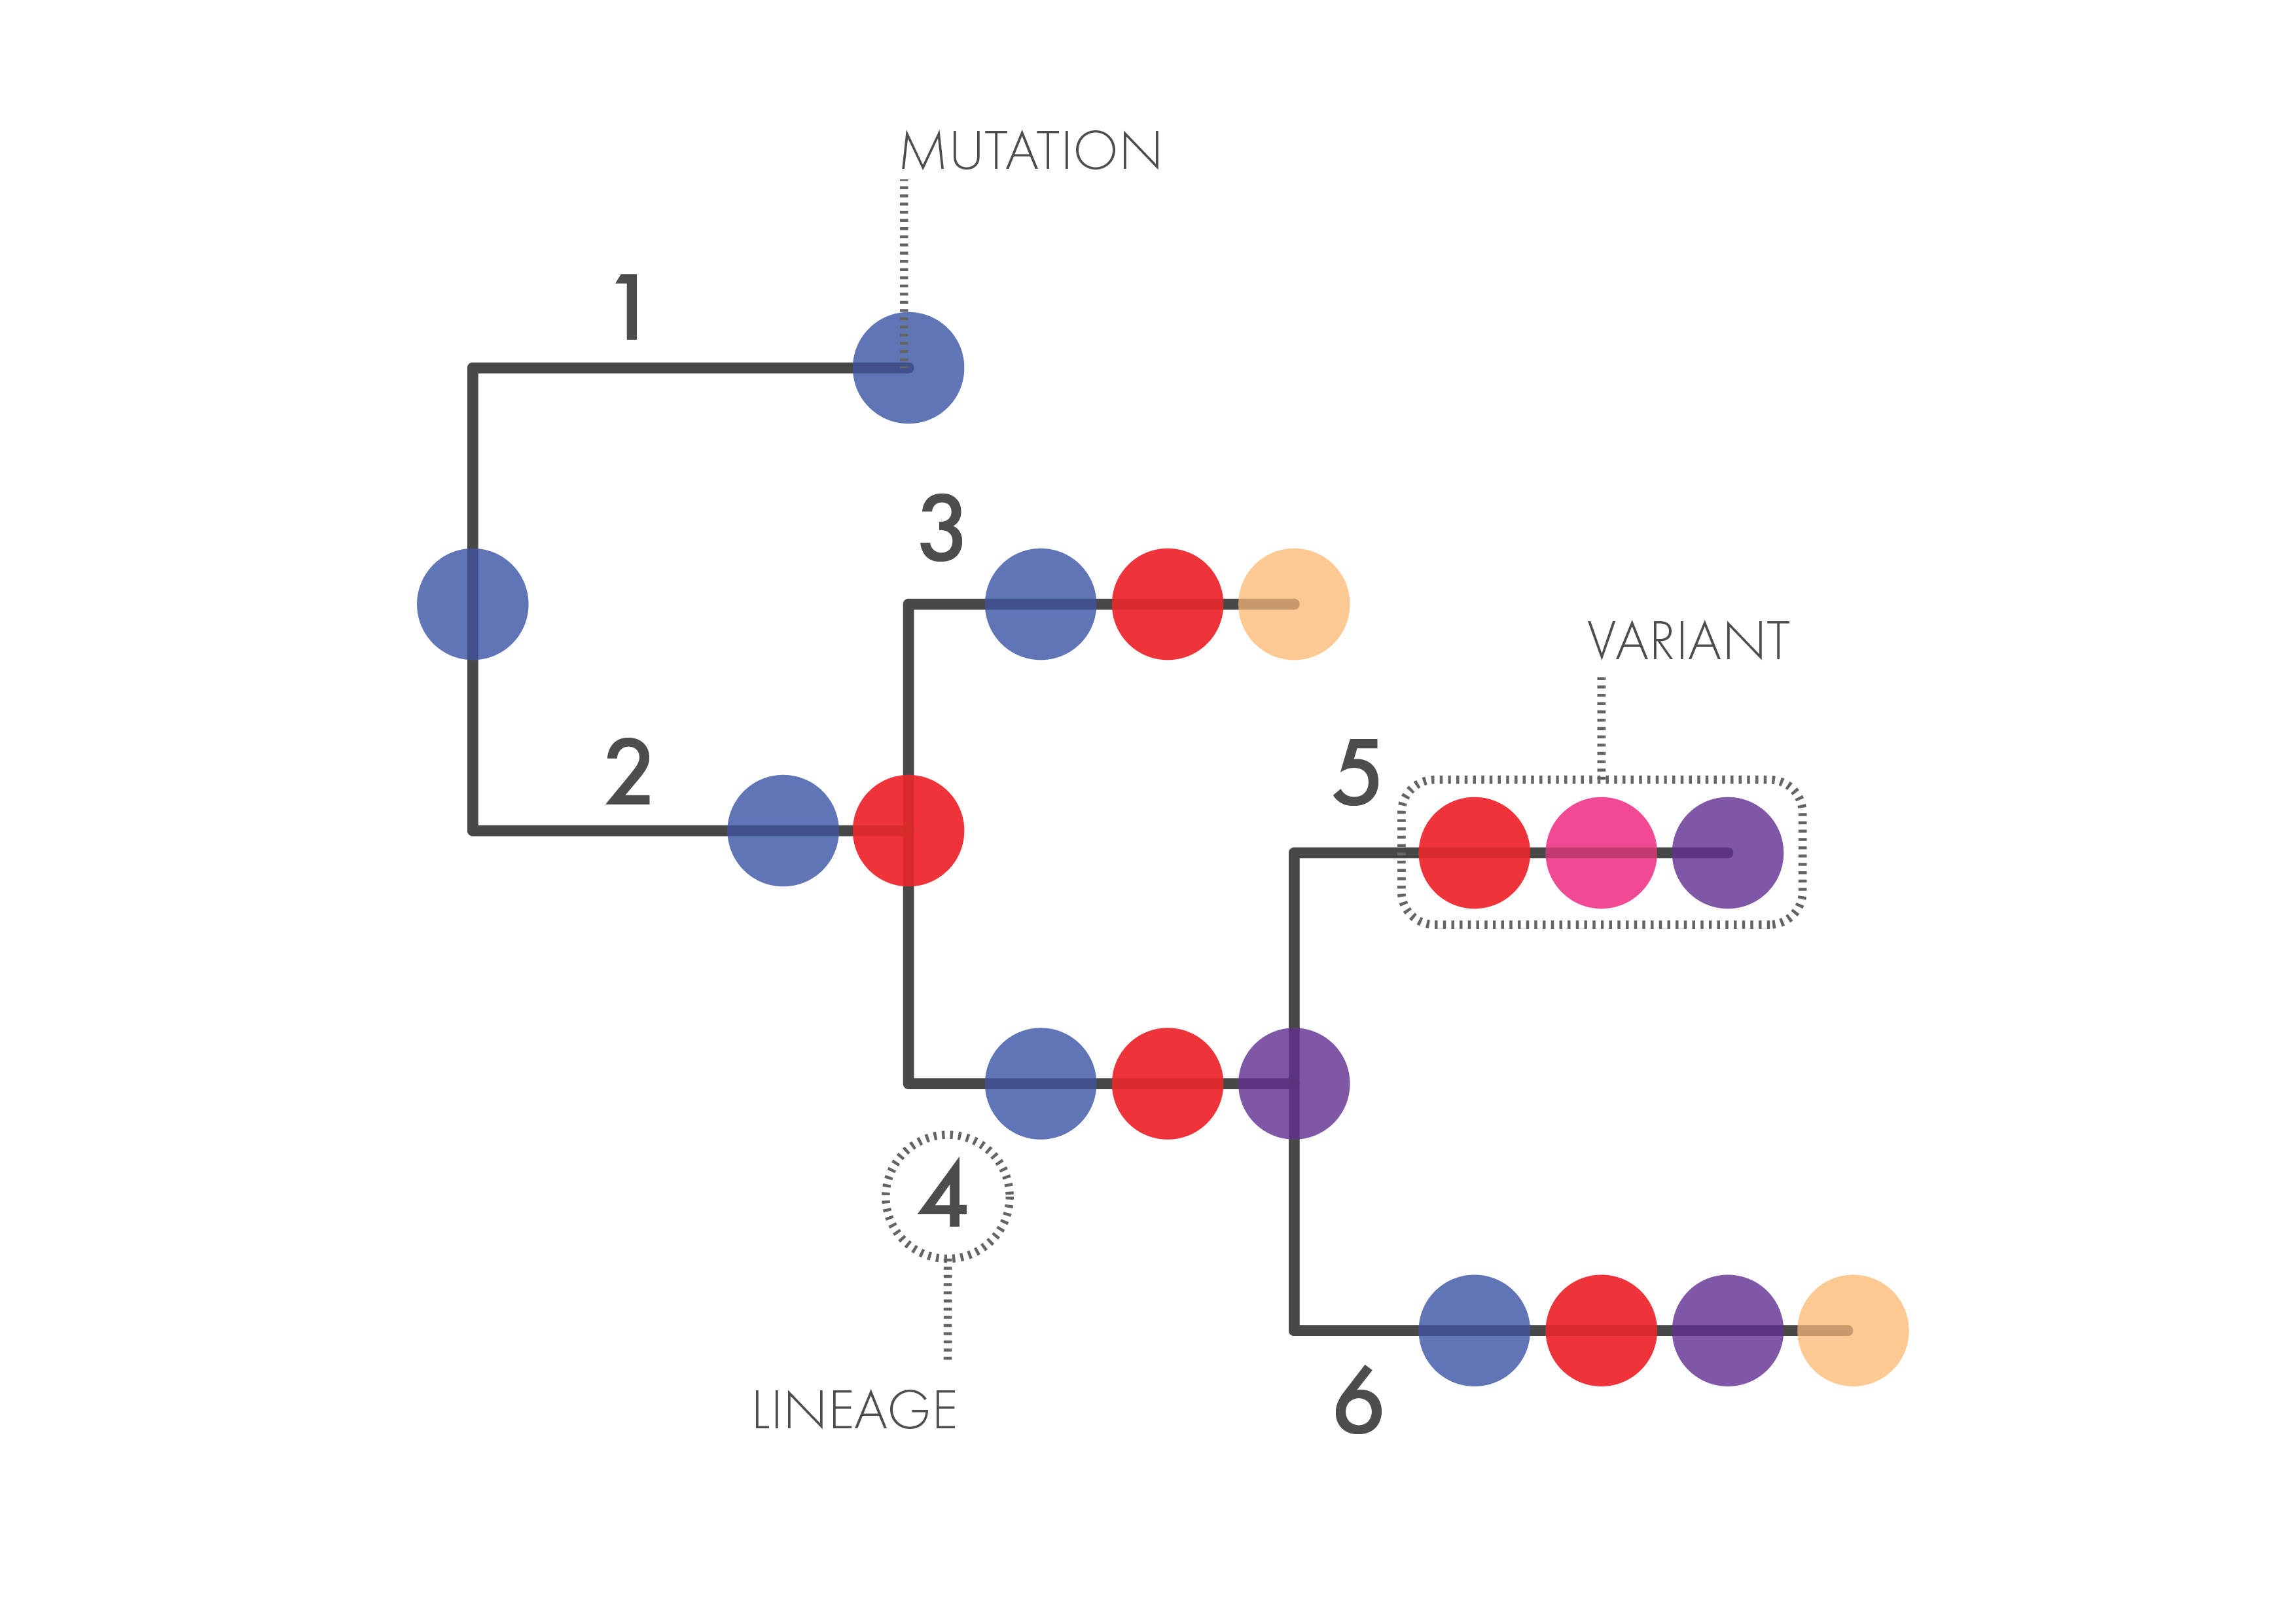
\includegraphics[width=0.5\textwidth]{images/fig2-terminology.jpg}
    \caption{Glossary of Mutations Terms}
    \label{fig2}
\end{figure}

The genome of the SARS-Cov2 virus is a 30 kb long (RNA virus) and like all living organisms the virus is subject to natural selection and it changes. Although this virus has multiple coding regions and each plays a key role when it comes to replication of the virus, I decided to look at all the variants that occur in the \textbf{S gene} of the virus, known as the \textit{glycoprotein} (or Spike protein).
The selection of this gene is based on its importance \cite{ref11} to the binding of the host cell. The first contact that a cell has with a viral particle is directed by this gene and its understanding its rate of mutation is potentially crucial. 


\subsection{Data acquisition}

The proposed idea of building a grammar in a way modeled the dataset, its final appearance is a result of the way these models learn and train. For the part of creating a dataset with biologically correct variants, huge acknowledgement goes to the GISAID platform \cite{ref12}, who have made tremendous effort to organize the data and create beautiful documentation of its features. 
There are several sections on the main GISAID website and all of them can be useful in some way for the dataset creation. Since our main focus was variants, the data was from the "Emerging Variants" section. This section of the page helps to monitor new variants of COVID-19 that may become relevant due to signs of increased proliferation (estimated by changing the number of sites) in combination with potential effects on receptor or antibody binding, commented in CoVsurver \cite{ref13}. Currently, 124 amino acid changes and glycoprotein (Spike) deletions occurring in at least 10 different geographic locations have been identified in studies to induce antibody escape, increased ACE2 \cite{ref14} binding, or increased protein expression and stability. Spike proteins are considered as part of the formation of combinations of potential variants to be followed.

\begin{figure}[h]
    \centering
    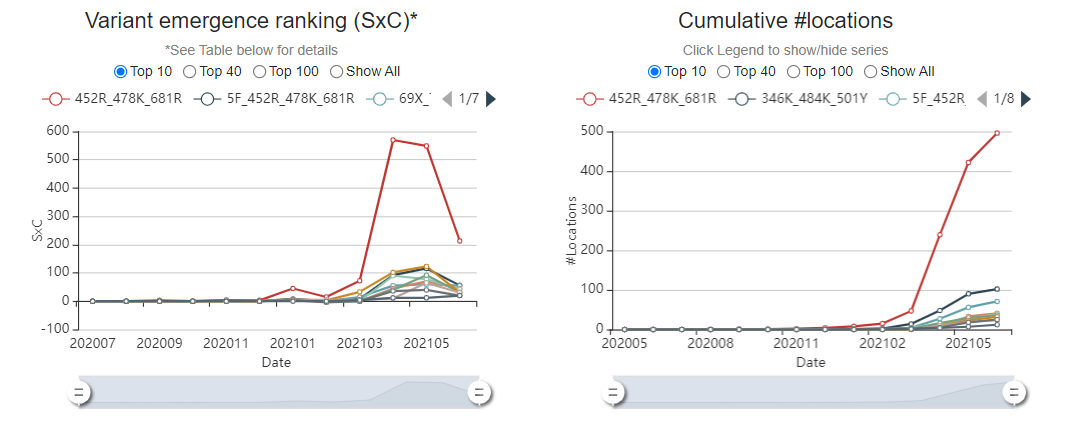
\includegraphics[width=0.485\textwidth]{images/fig3-variants_ranking.png}
    \caption{Variant emergence ranking (SxC) (left), Number of cumulative locations (right); GISAID}
    \label{fig3}
\end{figure}


Changes showed in Figure 3, that are with the "X" extension are undefined basics of the corresponding pages, which may also include Spike delete pages. The variants for each month (according to the date of collection) are ranked according to SxC, which is the product of the change in the number of sites (compared to previous months; similar to the spread of S) and the number of relevant amino acid changes with potential effect to combinations (C). 
\hspace{0pt}

The page itself has metadata for each month starting from July 2020 - April 2021. The data is organized in tables for each month separately where there is a larger number of columns (some of which are features in our dataset) and one such table can been seen in Figure 4. 

\begin{figure}[h]
    \centering
    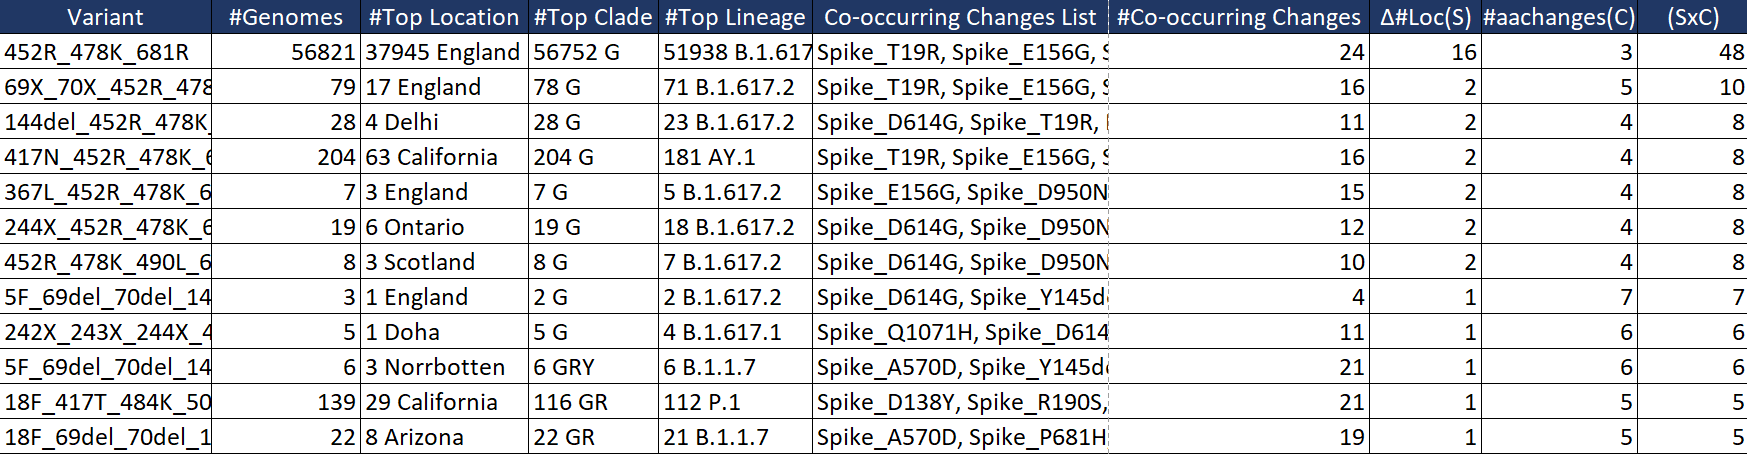
\includegraphics[width=0.485\textwidth]{images/fig4-dataset.png}
    \caption{First rows of emerging variants table for July 21'}
    \label{fig4}
\end{figure}

Each of the columns represents a potential information for learning models but we use a reduce the columns dataset, to the following columns: 

\begin{itemize}
\item \textbf{Variant} (string): The name is a combination of the amino acid changes and deletions in the Spike protein that occur in at least 10 different geographical locations and were identified in studies to cause antibody escape, increase ACE2 binding or increase Spike protein expression and stability are considered as part of combinations or constellations forming potential variants to be monitored. These 147 aa changes are the ones found in this "Variant" column
\item \textbf{Top Lineage} (number + string): Lineage values are the lineage (origin) of each new variant. The lineages are all from the PANGO \cite{ref15} platform and in the column are consisted of two parts:
    \begin{itemize}
    \item Largest number of sequenced genomes from this lineage from all genomes 
    \item Name of the PANGO lineage
    \end{itemize}
\item \textbf{Co-occurring changes} (list of strings): This is a list of all other amino acid changes that co-occur in  more than 75\% of all isolates with the variant (combinations of mutations) in the "Variant" column and are listed in this "Co-occurring changes" column. This list contains mutations not only for the glycoprotein but for the other genes of the genome as well (NSP, M etc.) These mutations that are found from GISAID may still be interesting to researchers who are tracking other possible contributing characteristics to these variants. Each element of the list is consisted of: 
\begin{itemize}
    \item  \textit{Protein name} (Spike or other proteins) = In which gene did the change in the virus genome occur (this is the same for everyone)
    \item  \textit{Amino acid in reference genome} = As in the example above, the first row has T
    \item  \textit{Position in glycoprotein sequence} = As in the example above, the first row has 19, that is the 19th position in the original glycoprotein
    \item \textit{Mutated protein in the new variant} = As in the example above, the first row has R, which means that if there is T19R it means that the protein T at position 19 is replaced by R in this variant
\end{itemize}
\item \textbf{(SxC)} (int): Product of the change in the number of sites (Loc or short S) and the number of relevant amino acid changes with potential effect (aachanges or short C)

\item \textbf{Timestamp} (string): Month and year for the variant 
\end{itemize}

\subsection{Data analysis}
The approach that is used to build a gramar from the data is based on a famous technique from the filed of Natural Language Processing called \textbf{Transformers}. \cite{ref16} The idea is to feed a bunch of "sentences" to this type of model in order for it to effectively learn which is a biologically logical (for it is logical grammar) amino acid. So, in order to do that we have to create:
\begin{itemize}
    \item list of all completely unique emerging variants
    \item list of unique lineages
\end{itemize}

\begin{figure}[h]
    \centering
    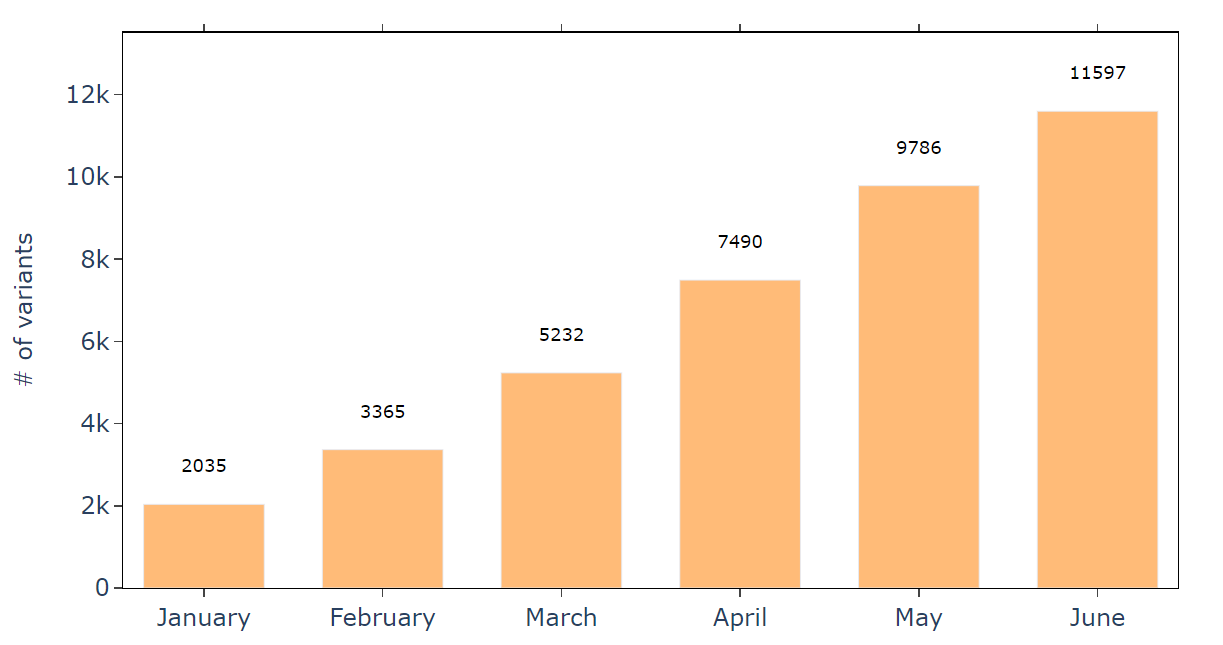
\includegraphics[width=0.47\textwidth]{images/fig5-number-variants.png}
    \caption{Number of variants per month}
    \label{fig5}
\end{figure}

The tables for each month are like the one displayed with Figure 4, and are in a period from July 20 '- June 21' (11 months in total). Figure 6 shows the total number of variants registered for months January 21' - June 21' and we can see that even after a year after the pandemic has started, the numbers between months have a linear growth. From January 21' - 2 035 it jumps to a frightening 11 597 in June 21', which only back ups the common genetic beliefs \cite{ref17} that RNA viruses mutate a very often. 

The total number of variants for the final dataset resulted in 11 937, and out of those variants only 2 224 are completely different. The reason for this reduced number of variants, after getting rid of the duplicates is that most of the variants are often separated into new emerging variants due to mutations to the other genes (proteins), not only the glycoprotein. Since the approach in this paper is to train a model that can distinctly tell apart amino acids of the S-gene, that is why we reduce the number of variants. 

\begin{figure}[h]
    \centering
    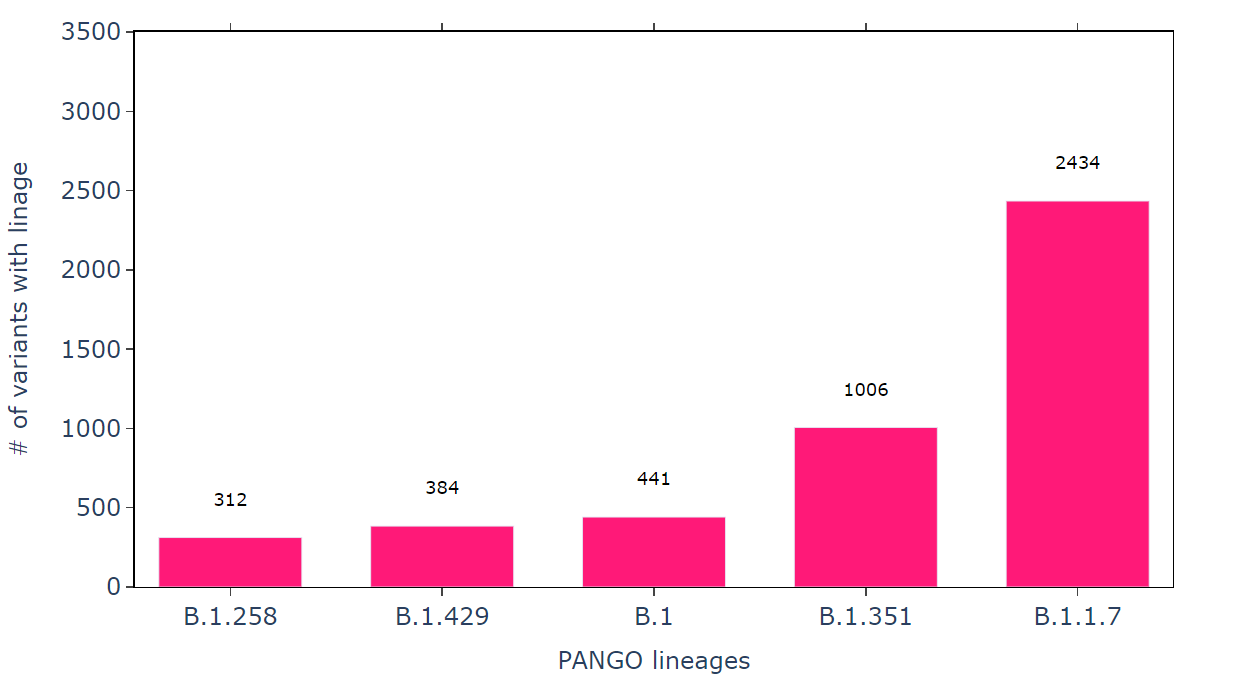
\includegraphics[width=0.485\textwidth]{images/fig6-common_linages.jpg.png}
    \caption{Five most common lineages}
    \label{fig6}
\end{figure}

After analysing all of the variants we then read the reference gene for each variant and mutate it on the positions based from the "Variant" column and "Co-occurring changes list" column. Afterwards we write them in our first smaller training dataset. But, all of these variants have their most common lineage, which is the second value inside the cells from the "Top lineage" column. This column had a major data flaws because most of the rows had wrong values (non-existing lineages) and if total number of lineages is same as the number of variants (11 397) after getting rid of all the duplicates and nonsense inputs the total number of unique lineages came up to 101. Figure 6 and Figure 7 showcases the 5 most common lineages, with the number of their occurrences and an alignment chart. 

\begin{figure}[h]
    \centering
    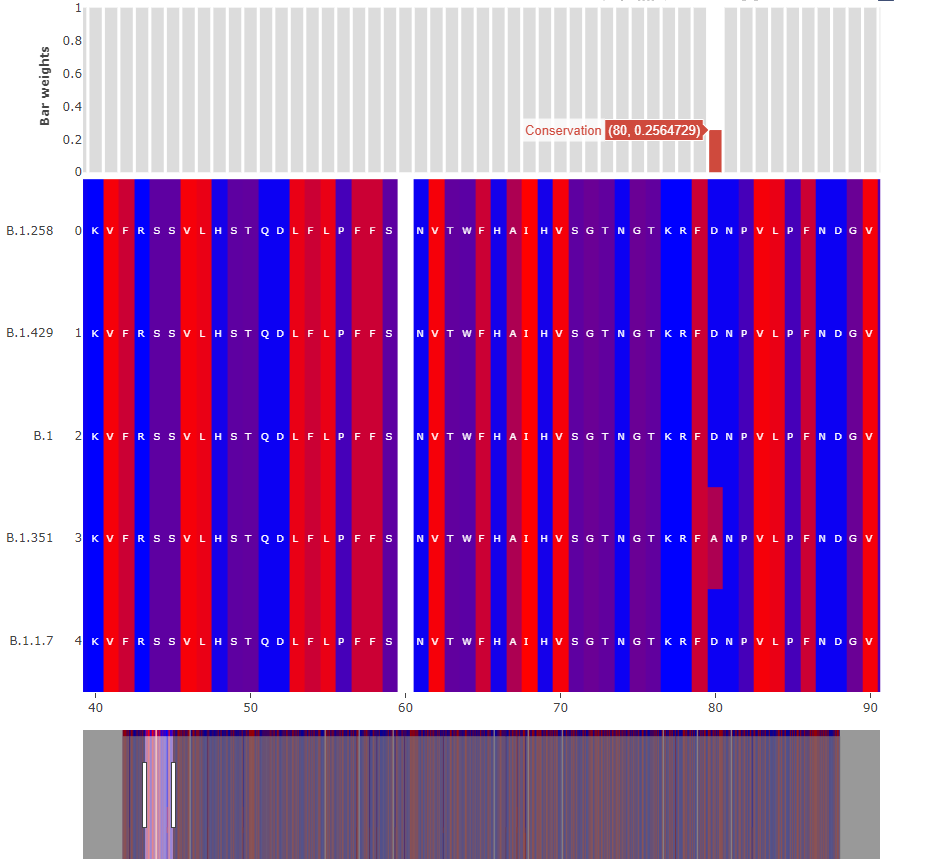
\includegraphics[width=0.485\textwidth]{images/fig7-aligment_chart.png}
    \caption{Alignment chart of the five most common lineages (range base pairs 40-90)}
    \label{fig7}
\end{figure}

In the number of total occurrences the clear leader is the linage B.1.17 \cite{ref18} commonly know as the \textit{Alpha variant}. 
As of 4 July 2021, 962,104 sequences in the B.1.1.7 lineage have been detected \cite{ref19}. It was first identified in the UK in September 2020 and has since been detected in the US \cite{ref20} and other countries. This variant is of growing concern because it has shown to be significantly more transmissible than other variants. 


The analysis of the lineages finished with a search of all of the mutations since they are not included in our dataset. However,  the Center for Viral Systems Biology (outbreak.info) \cite{ref21} has all of the lineages and their mutations written in JSON files. After manually downloading all of the files, the last step is to mutate all of the amino acids in the reference genome peptide and write them all into our second smaller dataset. After this step the final dataset is consisted of \textbf{2 325 samples}. 


\section{Methods}

The current dataset is just RNA sequences, that are read at the input of the model (from the S-gene region: 21563-25384).
Although the problem can be solved by classification, for example getting a value for the Sxc column like a score this method gives creates a grammar which is a different approach. 

\subsection{Transformers architecture}
Transformer models are based on sequence-to-sequence architecture (Seq2Seq), that has been used frequently in the world of natural language processing (NLP). \cite{ref22,ref23}  In the background, there is a neural network that transforms a given sequence of elements, a sequence of words into a sentence, and transforms it into a new sequence - sentence.
However, these models are primarily used for translation from one language to another, their way of learning led to the idea proposed in this article.
Seq2Seq models are composed of \textit{Encoder} and \textit{Decoder}. The encoder reads an input sequence and maps it to a multidimensional vector. This abstract vector then feeds the Decoder which transforms it into an output sequence. This output can be in another language, symbol, copy of the input itself, etc.
When I imagine the model, it reminds me of the following scenario: Encoder and Decoder speak two languages, one is their mother tongue different for both (for example German and Macedonian) while their second is an imaginary language and common to both. To translate something from German to Macedonian, the Encoder must convert from a German sentence to an imaginary one, and then the Decoder reads that imaginary one and translates it into Macedonian.

\begin{figure}[h]
    \centering
    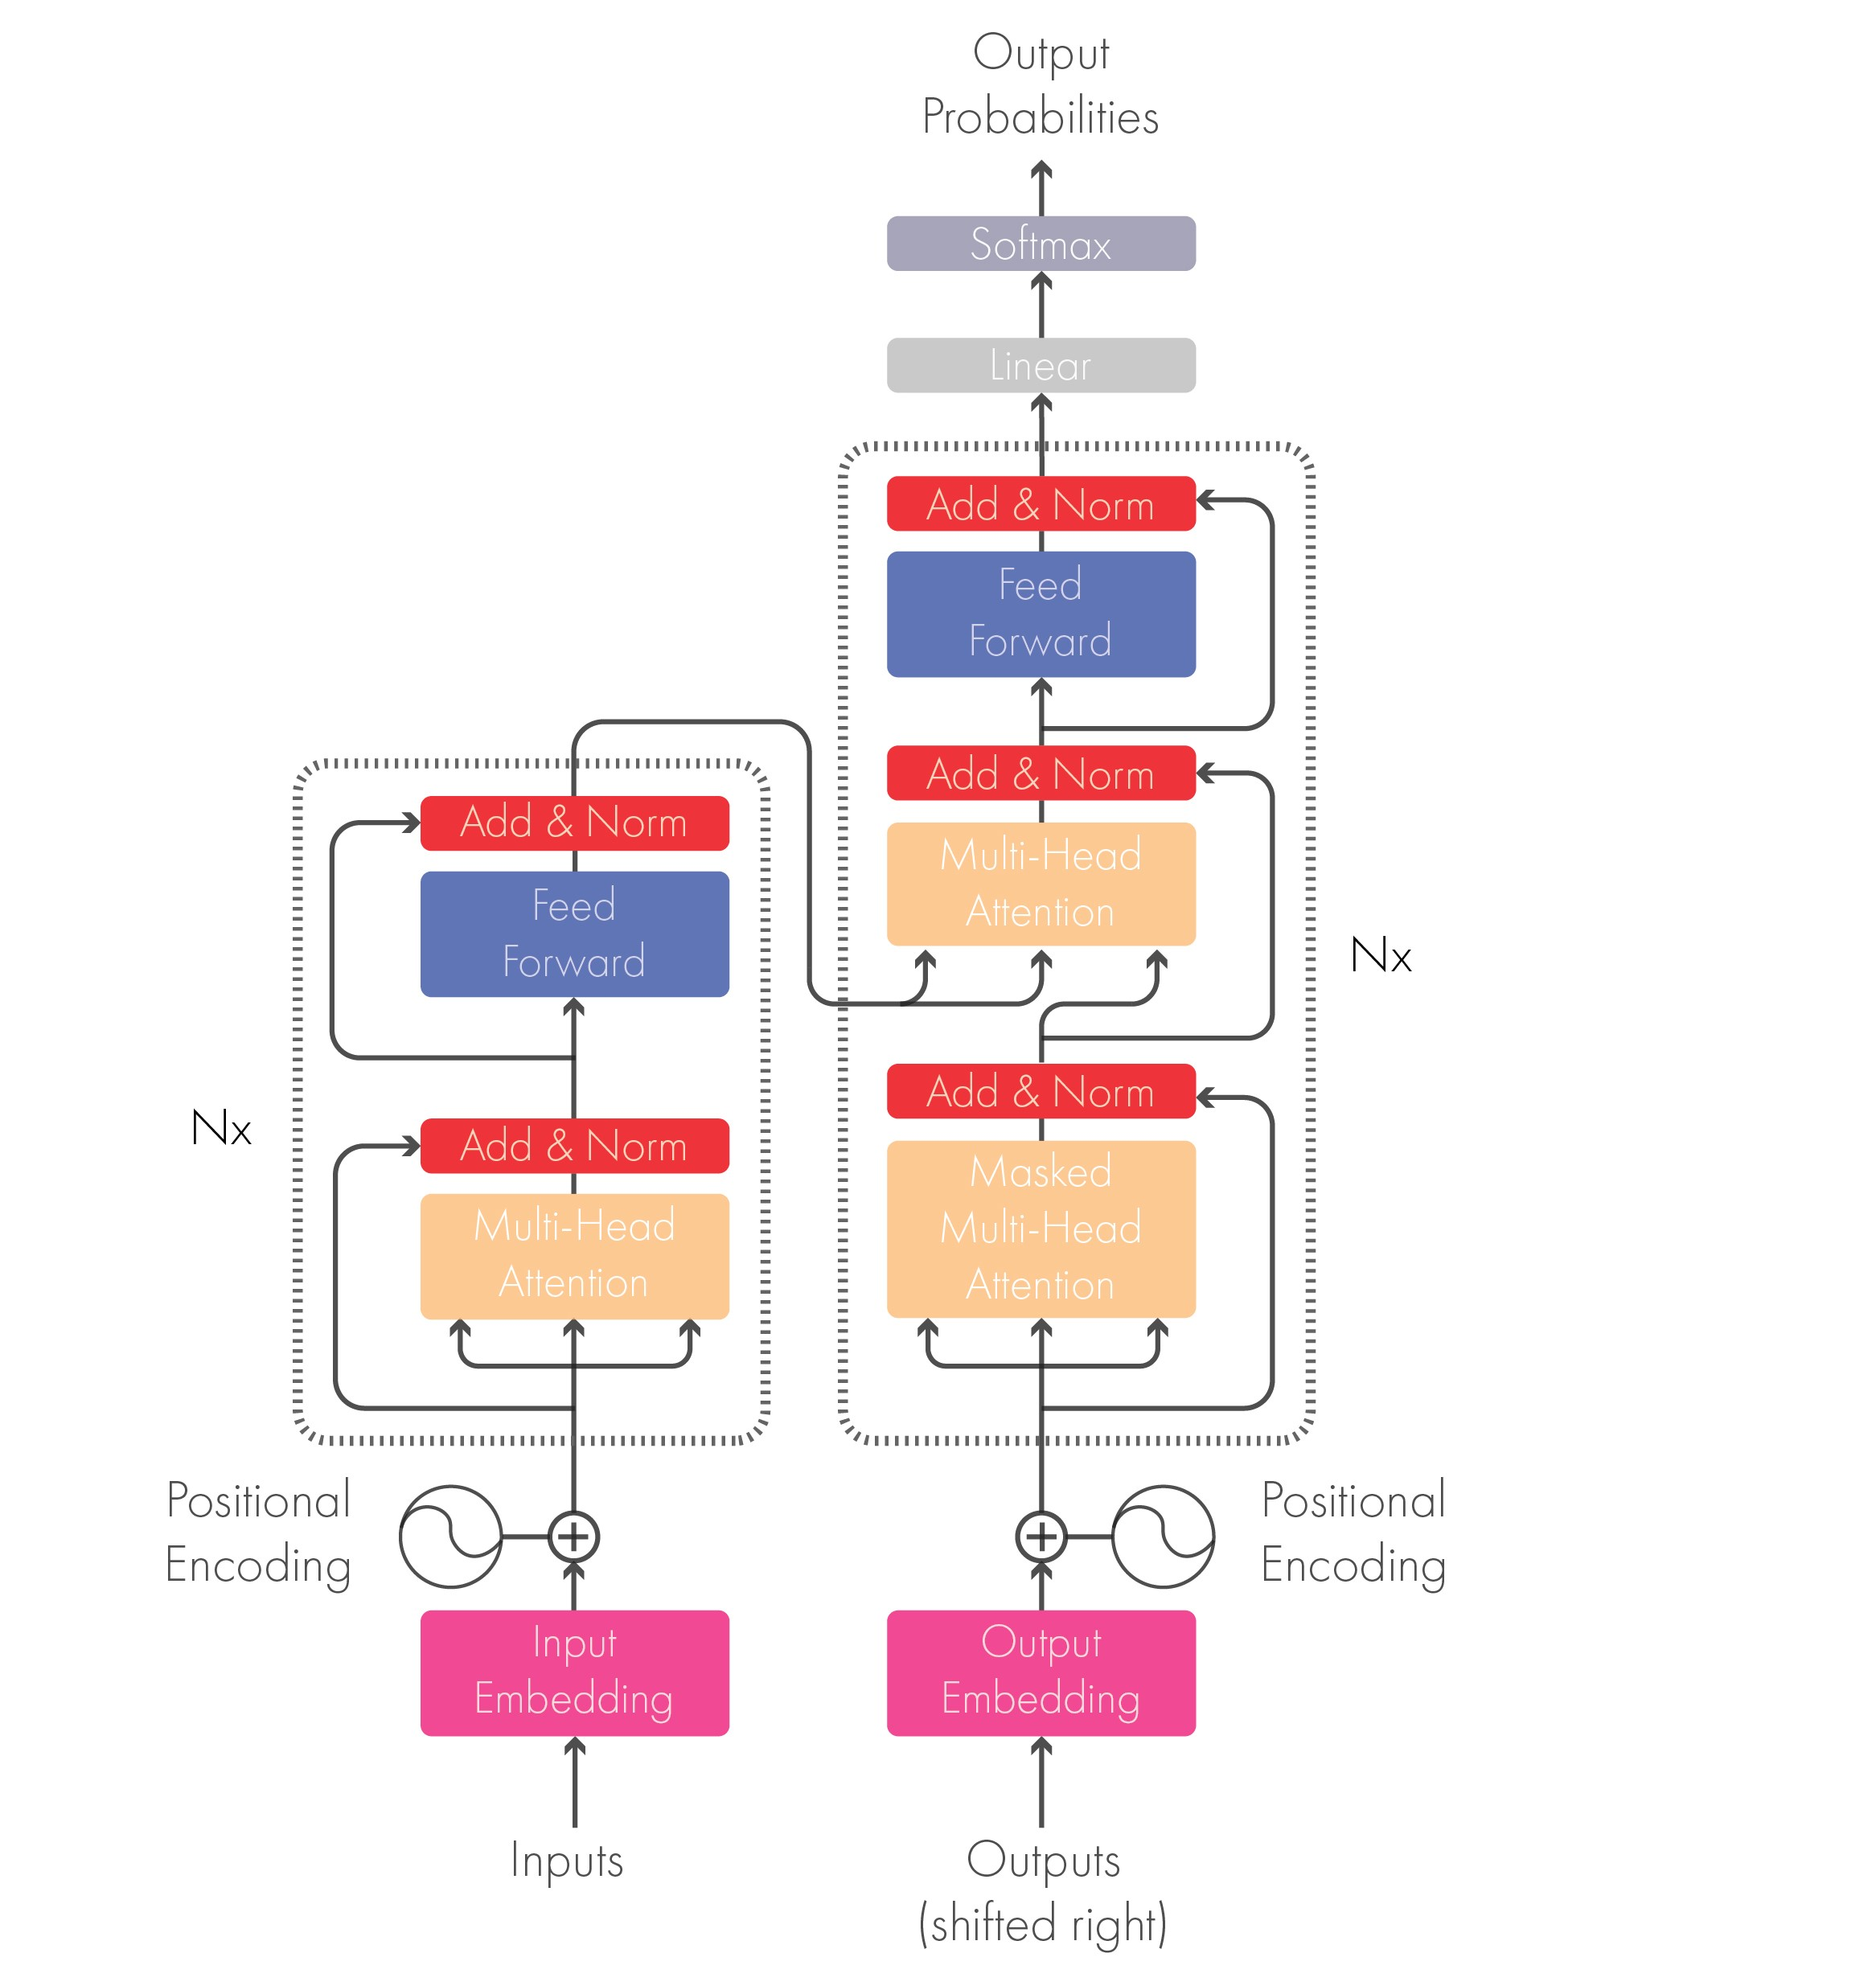
\includegraphics[width=0.485\textwidth]{images/fig8-architecture.jpg}
    \caption{The Transformer model architecture \cite{ref24}}
    \label{fig8}
\end{figure}

Now why are languages and this whole method useful for predicting virus variants? The answer is again a question: How do we know which part of the sequence is subject to change in the next variant?
And here this is solved by the very way architecture teaches. If we imagine a scenario where neither the Encoder nor the Decoder have a common imaginary language, in order to learn it they have to train (the model is trained) with many samples. A simple choice for Encoder and Decoder from such an architecture are single LSTMs for each of the two. 

\subsection{Attention}

The paper ‘Attention Is All You Need’ \cite{ref24} is probably the best introduction to the novel architecture called Transformer. As the title indicates, it uses the attention-mechanism we saw earlier. Like LSTM, Transformer is an architecture for transforming one sequence into another one with the help of two parts (Encoder and Decoder), but it differs from the previously described/existing sequence-to-sequence models because it does not imply any Recurrent Networks (GRU, LSTM, etc.).

To make the transformers easier to understand, there is one technical detail that is very important to complement the idea and that is the \textit{attention detail}.
The attention mechanism of the model itself looks at the input sequence and decides at each step of learning which other parts of the sequence are important. This sounds a bit abstract, but a simple example helps:
When you read this sentence, you always focus on the word you are reading but at the same time your mind keeps all the content of the most important keywords in memory so that it can give meaning and not be random.

\begin{equation}
Attention(Q, K, V) = softmax(\frac{QK^{T}}{\sqrt{d_k}}) V
\end{equation}

This mechanism works similarly to the sequence. For example, if we are talking about the translation from above, then this mechanism would be the Encoder when translating writes keywords related to the translation that are important for the semantics, and passes them to the Decoder as a plus before starting to translate. These new words make the Decoder's job easier because he knows exactly which parts of the sentence are important so that the context is not lost.
Thus, in the learning process, the models put masks (context labels) that are placed on the input sequence itself in the first as a multi-head, and this is actually done to avoid potential "future" errors with the elements of the sequence ( more about this in the other stages).
These masks would be the mutations themselves for the input variant, which is our feature in the set of input sequences, and we place them so that the decoder can learn accurately in those places about the future sequence.

\hspace{0pt}

Let’s start with the description of the attention-mechanism. It’s not very complicated and can be described by equation (1). $Q$ is a matrix that contains the query (vector representation of one word in the sequence), K are all the keys (vector representations of all the words in the sequence) and $V$ are the values, which are again the vector representations of all the words in the sequence. For the encoder and decoder, multi-head attention modules, $V$ consists of the same word sequence than $Q$. However, for the attention module that is taking into account the encoder and the decoder sequences, $V$ is different from the sequence represented by $Q$.

After the multi-attention heads in both the encoder and decoder, we have a pointwise feed-forward layer. This little feed-forward network has identical parameters for each position, which can be described as a separate, identical linear transformation of each element from the given sequence.

\subsection{Training}
How to train such a ‘beast’? Training and inferring on Seq2Seq models is a bit different from the usual classification problem. The same is true for Transformers.

Thus in the training process, the models put masks (context labels) that are placed on the input sequence itself in the first as a multi-head, and this is actually done to avoid potential "future" errors with the sequence elements.
These masks would be the mutations themselves for the input variant, which is our feature in the set of input sequences, and we place them in order for the decoder to learn accurately in those places about the future sequence.

We are training a new language model from scratch using the Python libraries \textit{Transformers} and \textit{Tokenizers}. We choose to train a byte-level Byte-pair encoding tokenizer (the same as GPT-2), with the same special tokens as RoBERTa \cite{ref25}. We then pick a vocabulary size of 22 (20 amino acids + token for a beginning and an end). After the vocabulary is set the library saves both a vocab.json, which is a list of the most frequent tokens ranked by frequency, and a merges.txt list of merges. After this the last couple of steps are tokenizing the inputs and spliting the dataset with a  85 (train) - 15 (eval) split, having 1977 samples for training and 348 for evaluation loss. 

\section{Results}
For trainging the model we used a Google \textit{Colab enviroment} \cite{ref26}, with a Nvidia K80s, with 24 GB of GDDR5 memory. The training took 2h 12min
to complete and resulted with a evaluation loss of only 6\% ($evaluation loss=0.0655$). 

\begin{figure}[h]
    \centering
    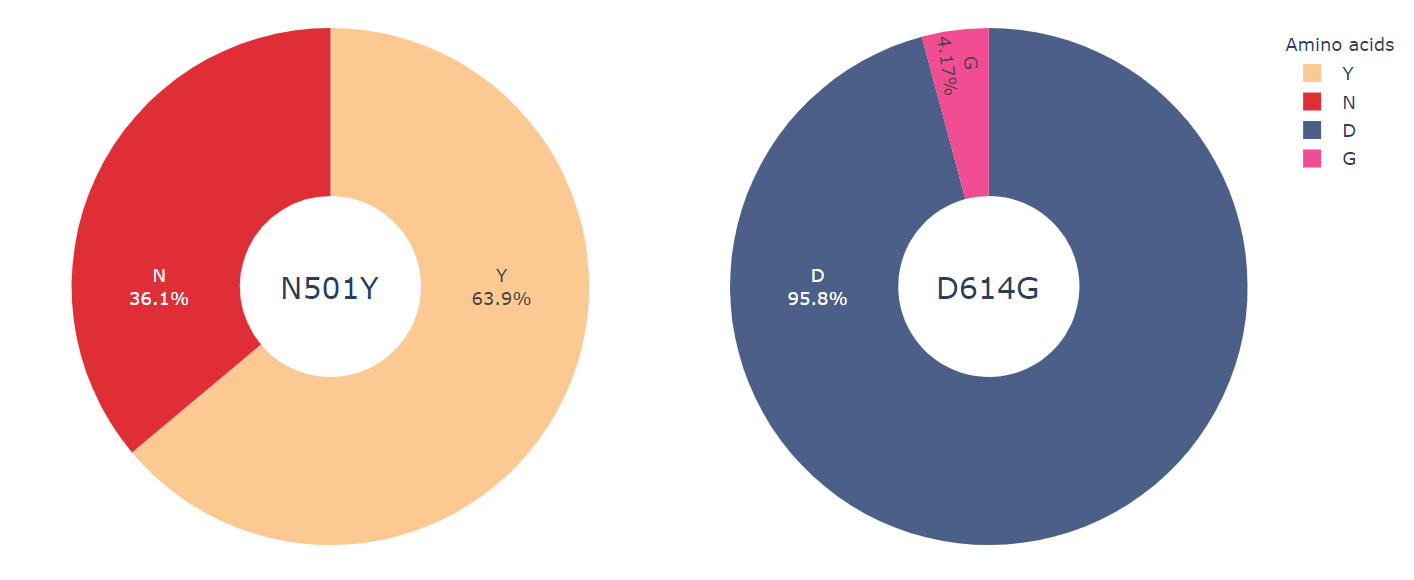
\includegraphics[width=0.48\textwidth]{images/fig9-freq_mutations.png}
    \caption{Frequency of amino acid in dataset sequences at locations 501 and 614 in the Spike protein}
    \label{fig9}
\end{figure}


Aside from looking at the training and eval losses going down, the easiest way to check whether our language model is learning anything interesting is via the \textit{FillMaskPipeline}. Pipelines are simple wrappers around tokenizers and models, and the 'fill-mask' one will let you input a sequence containing a masked token (here, <mask>) and return a list of the most probable filled sequences, with their probabilities. 


Now we start masking the amino acids locations we desire to see and see if our model captures them. We started by masking the first location, 0 which is 100\% the amino acid M, and our model caught it with a $prob score=0.9999$. But, this was an easy one so we tried testing one of the 2 most lethal mutations \cite{ref27}, which are the N501Y and the D614G. 

\begin{figure}[h]
    \centering
    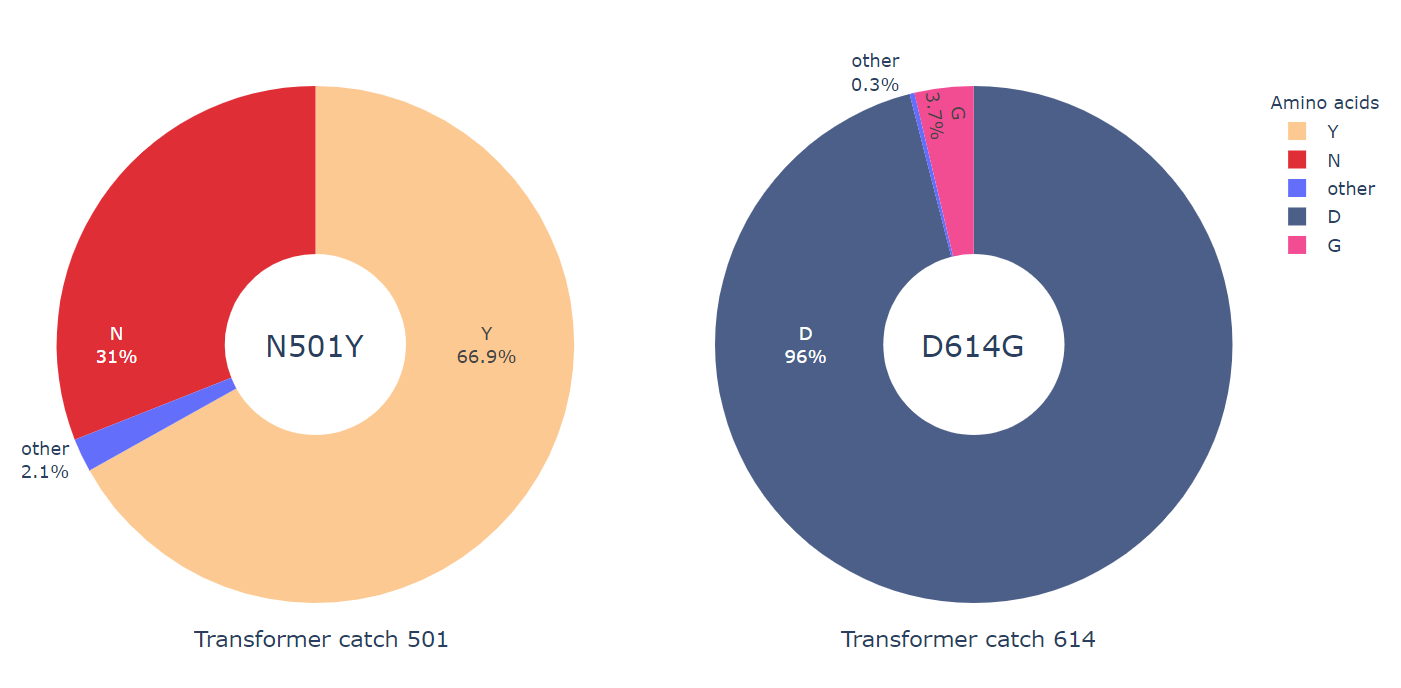
\includegraphics[width=0.48\textwidth]{images/fig10-freq_transformer.png}
    \caption{Transformer catches for frequency of amino acid in dataset sequences at locations 501 and 614 in the Spike protein}
    \label{fig10}
\end{figure}


Figure 9 shows their frequency calculated from our sequences dataset.The scores that the model returned are displayed in Figure 10, and prove this approach can be promising for potentially catching mutations in the Spike protein. The frequency of our dataset scores N with 63.9\% and Y with 36.1 \%, while he viral transformer scores N with 66.9\% and Y with 31\%. 


\section{Discussion}
The Transformer model has truly changed the way we work with text data and has yet a chance to prove itself for usages outside the world of language processing. Although it is considered only as a tool for translation, this moderate attempt to catch mutations and build a vocabualry has shown that the capabilitites of this architecture are remarkable. The results may be a little bias on the input that we feed it, but to have such a small evaluation loss and still beeing able to catch with close accuracy the mutations justified our approach and hypothesis that NLP has a place in the Genetics world. Although this is a modest attempt to process natural languages, the next step would be to mix Transformers and GAN networks \cite{ref28} to create larger datasets in order to predict not only catch new variants. GAN networks have been proven to stamp new biologically sequences \cite{ref29} and similar models have been successful as well. Let these results paint an  interesting picture about how  easily different fields can mix and match to create better understanding of totally distinct problems. 

% conference papers do not normally have an appendix





% trigger a \newpage just before the given reference
% number - used to balance the columns on the last page
% adjust value as needed - may need to be readjusted if
% the document is modified later
%\IEEEtriggeratref{8}
% The "triggered" command can be changed if desired:
%\IEEEtriggercmd{\enlargethispage{-5in}}

% references section

% can use a bibliography generated by BibTeX as a .bbl file
% BibTeX documentation can be easily obtained at:
% http://mirror.ctan.org/biblio/bibtex/contrib/doc/
% The IEEEtran BibTeX style support page is at:
% http://www.michaelshell.org/tex/ieeetran/bibtex/
%\bibliographystyle{IEEEtran}
% argument is your BibTeX string definitions and bibliography database(s)
%\bibliography{IEEEabrv,../bib/paper}
%
% <OR> manually copy in the resultant .bbl file
% set second argument of \begin to the number of references
% (used to reserve space for the reference number labels box)
\begin{thebibliography}{1}

\bibitem{ref1}
K. Yuen, Z. Ye, S. Fung, C. Chan and D. Jin, "SARS-CoV-2 and COVID-19: The most important research questions", Cell \& Bioscience, vol. 10, no. 1, 2020. Available: 10.1186/s13578-020-00404-4 [Accessed 5 July 2021].

\bibitem{ref2}
"outbreak.info", outbreak.info, 2021. [Online]. Available: https://outbreak.info/situation-reports?pango=B.1.1.7\&loc=GBR\&loc=USA\&loc=USA\_US-CA\&selected=GBR. [Accessed: 01- Jun- 2021].


\bibitem{ref3}
"Will the Coronavirus Ever Go Away? Here's What a Top WHO Expert Thinks", Time, 2021. [Online]. Available: https://time.com/5805368/will-coronavirus-go-away-world-health-organization/. [Accessed: 01- Jun- 2021].

\bibitem{ref4}
I. Korolev, "Identification and estimation of the SEIRD epidemic model for COVID-19", Journal of Econometrics, vol. 220, no. 1, pp. 63-85, 2021. Available: 10.1016/j.jeconom.2020.07.038 [Accessed 5 July 2021].

\bibitem{ref5}
G. Mahmoudabadi and R. Phillips, "A comprehensive and quantitative exploration of thousands of viral genomes", eLife, vol. 7, 2018. Available: 10.7554/elife.31955 [Accessed 5 July 2021].

\bibitem{ref6}
R. Plowright et al., "Pathways to zoonotic spillover", Nature Reviews Microbiology, vol. 15, no. 8, pp. 502-510, 2017. Available: 10.1038/nrmicro.2017.45 [Accessed 5 July 2021].

\bibitem{ref7}
"Severe acute respiratory syndrome coronavirus 2 isolate Wuhan-Hu-1, co - Nucleotide - NCBI", Ncbi.nlm.nih.gov, 2021. [Online]. Available: https://www.ncbi.nlm.nih.gov/nuccore/NC\_045512.2/. [Accessed: 05- Jul- 2021].

\bibitem{ref8}
[8] www.dw.com), "India tops 200,000 dead amid coronavirus surge | DW | 28.04.2021", DW.COM, 2021. [Online]. Available: https://www.dw.com/en/india-tops-200000-dead-amid-coronavirus [Accessed: 05- Jul- 2021].

\bibitem{ref9}
"Covid: Brazil has more than 4,000 deaths in 24 hours for first time", BBC News, 2021. [Online]. Available: https://www.bbc.com/news/world-latin-america-56657818. [Accessed: 07- Apr- 2021].

\bibitem{ref10}
T. Schlub et al., "Fifteen to Twenty Percent of HIV Substitution Mutations Are Associated with Recombination", Journal of Virology, vol. 88, no. 7, pp. 3837-3849, 2014. Available: 10.1128/jvi.03136-13 [Accessed 5 July 2021].

\bibitem{ref11}
K. Holmes and R. Williams, "Background Paper Functions of Coronavirus Glycoproteins", Advances in Experimental Medicine and Biology, pp. 5-7, 1990. Available: 10.1007/978-1-4684-5823-7\_2 [Accessed 5 July 2021].

\bibitem{ref12}
Elbe, S., and Buckland-Merrett, G. (2017) Data, disease and diplomacy: GISAID's innovative contribution to global health. Available: https://www.gisaid.org/

\bibitem{ref13}
"GISAID - CoVsurver mutations App", Gisaid.org, 2021. [Online]. Available: https://www.gisaid.org/epiflu-applications/covsurver-mutations-app/. [Accessed: 05- Jul- 2021].

\bibitem{ref14}
X. Xue et al., "Dynamics of binding ability prediction between spike protein and human ACE2 reveals the adaptive strategy of SARS-CoV-2 in humans", Scientific Reports, vol. 11, no. 1, 2021. Available: 10.1038/s41598-021-82938-2 [Accessed 5 July 2021].

\bibitem{ref15}
A. Rambaut et al., "Addendum: A dynamic nomenclature proposal for SARS-CoV-2 lineages to assist genomic epidemiology", Nature Microbiology, vol. 6, no. 3, pp. 415-415, 2021. Available: 10.1038/s41564-021-00872-5.

\bibitem{ref16}
H. Models, "Transformers In NLP | State-Of-The-Art-Models", Analytics Vidhya, 2021. [Online]. Available: https://www.analyticsvidhya.com/blog/2019/06/understanding-transformers-nlp-state-of-the-art-models/. [Accessed: 05- Jul- 2021].

\bibitem{ref17}
S. Duffy, "Why are RNA virus mutation rates so damn high?", PLOS Biology, vol. 16, no. 8, p. e3000003, 2018. Available: 10.1371/journal.pbio.3000003.

\bibitem{ref18}
N. Davies et al., "Estimated transmissibility and impact of SARS-CoV-2 lineage B.1.1.7 in England", Science, vol. 372, no. 6538, p. eabg3055, 2021. Available: 10.1126/science.abg3055 [Accessed 5 July 2021].

\bibitem{ref19}
"outbreak.info", outbreak.info, 2021. [Online]. Available: https://outbreak.info/situation-reports?pango=B.1.1.7\&loc=GBR\&loc=USA\&loc=USA\_US-CA\&selected=GBR. [Accessed: 05- Jul- 2021].

\bibitem{ref20}
Galloway SE, Paul P, MacCannell DR, et al. Emergence of SARS-CoV-2 B.1.1.7 Lineage — United States, December 29, 2020–January 12, 2021. MMWR Morb Mortal Wkly Rep 2021;70:95–99. Available: http://dx.doi.org/10.15585/mmwr.mm7003e2external icon

\bibitem{ref21}
Julia L. Mullen, Ginger Tsueng, Alaa Abdel Latif, Manar Alkuzweny, Marco Cano, Emily Haag, Jerry Zhou, Mark Zeller, Emory Hufbauer, Nate Matteson, Kristian G. Andersen, Chunlei Wu, Andrew I. Su, Karthik Gangavarapu, Laura D. Hughes, and the Center for Viral Systems Biology outbreak.info. Available: https://outbreak.info/ (2020)

\bibitem{ref22}
D. Schutte et al., "Discovering novel drug-supplement interactions using a dietary supplements knowledge graph generated from the biomedical literature", arXiv.org, 2021. [Online]. Available: https://arxiv.org/abs/2106.12741v1. [Accessed: 05- Jul- 2021]. 

\bibitem{ref23}
S. Pingali, S. Yadav, P. Dutta and S. Saha, "Multimodal Graph-based Transformer Framework for Biomedical Relation Extraction", arXiv.org, 2021. [Online]. Available: https://arxiv.org/abs/2107.00596. [Accessed: 05- Jul- 2021].

\bibitem{ref24}
A. Vaswani et al., "Attention Is All You Need", arXiv.org, 2021. [Online]. Available: https://arxiv.org/abs/1706.03762. [Accessed: 05- Jul- 2021].

\bibitem{ref25}
Y. Liu et al., "RoBERTa: A Robustly Optimized BERT Pretraining Approach", arXiv.org, 2021. [Online]. Available: https://arxiv.org/abs/1907.11692. [Accessed: 05- Jul- 2021].

\bibitem{ref26}
Bisong E. (2019) Google Colaboratory. In: Building Machine Learning and Deep Learning Models on Google Cloud Platform. Apress, Berkeley, CA. https://doi.org/10.1007/978-1-4842-4470-8\_7

\bibitem{ref27}
"The delta variant is the most dangerous SARS-CoV-2 mutation yet", The Economist, 2021. [Online]. Available: https://www.economist.com/graphic-detail/2021/06/16/the-delta-variant-is-the-most-dangerous-sars-cov-2-mutation-yet. [Accessed: 05- Jul- 2021].

\bibitem{ref28}
 I. Goodfellow et al., "Generative Adversarial Networks", arXiv.org, 2021. [Online]. Available: https://arxiv.org/abs/1406.2661. [Accessed: 05- Jul- 2021].
 
\bibitem{ref29}
D. Repecka et al., "Expanding functional protein sequence spaces using generative adversarial networks", Nature Machine Intelligence, vol. 3, no. 4, pp. 324-333, 2021. Available: 10.1038/s42256-021-00310-5 [Accessed 5 July 2021].

\end{thebibliography}




% that's all folks
\end{document}


